%<dscrpt>Fichier de déclarations Latex à inclure au début d'un élément de cours.</dscrpt>

\documentclass[a4paper]{article}
\usepackage[hmargin={1.8cm,1.8cm},vmargin={2.4cm,2.4cm},headheight=13.1pt]{geometry}

%includeheadfoot,scale=1.1,centering,hoffset=-0.5cm,
\usepackage[pdftex]{graphicx,color}
\usepackage[french]{babel}
%\selectlanguage{french}
\addto\captionsfrench{
  \def\contentsname{Plan}
}
\usepackage{fancyhdr}
\usepackage{floatflt}
\usepackage{amsmath}
\usepackage{amssymb}
\usepackage{amsthm}
\usepackage{stmaryrd}
%\usepackage{ucs}
\usepackage[utf8]{inputenc}
%\usepackage[latin1]{inputenc}
\usepackage[T1]{fontenc}


\usepackage{titletoc}
%\contentsmargin{2.55em}
\dottedcontents{section}[2.5em]{}{1.8em}{1pc}
\dottedcontents{subsection}[3.5em]{}{1.2em}{1pc}
\dottedcontents{subsubsection}[5em]{}{1em}{1pc}

\usepackage[pdftex,colorlinks={true},urlcolor={blue},pdfauthor={remy Nicolai},bookmarks={true}]{hyperref}
\usepackage{makeidx}

\usepackage{multicol}
\usepackage{multirow}
\usepackage{wrapfig}
\usepackage{array}
\usepackage{subfig}


%\usepackage{tikz}
%\usetikzlibrary{calc, shapes, backgrounds}
%pour la présentation du pseudo-code
% !!!!!!!!!!!!!!      le package n'est pas présent sur le serveur sous fedora 16 !!!!!!!!!!!!!!!!!!!!!!!!
%\usepackage[french,ruled,vlined]{algorithm2e}

%pr{\'e}sentation du compteur de niveau 2 dans les listes
\makeatletter
\renewcommand{\labelenumii}{\theenumii.}
\renewcommand{\thesection}{\Roman{section}.}
\renewcommand{\thesubsection}{\arabic{subsection}.}
\renewcommand{\thesubsubsection}{\arabic{subsubsection}.}
\makeatother


%dimension des pages, en-t{\^e}te et bas de page
%\pdfpagewidth=20cm
%\pdfpageheight=14cm
%   \setlength{\oddsidemargin}{-2cm}
%   \setlength{\voffset}{-1.5cm}
%   \setlength{\textheight}{12cm}
%   \setlength{\textwidth}{25.2cm}
   \columnsep=1cm
   \columnseprule=0.5pt

%En tete et pied de page
\pagestyle{fancy}
\lhead{MPSI-\'Eléments de cours}
\rhead{\today}
%\rhead{25/11/05}
\lfoot{\tiny{Cette création est mise à disposition selon le Contrat\\ Paternité-Pas d'utilisations commerciale-Partage des Conditions Initiales à l'Identique 2.0 France\\ disponible en ligne http://creativecommons.org/licenses/by-nc-sa/2.0/fr/
} }
\rfoot{\tiny{Rémy Nicolai \jobname}}


\newcommand{\baseurl}{http://back.maquisdoc.net/data/cours\_nicolair/}
\newcommand{\urlexo}{http://back.maquisdoc.net/data/exos_nicolair/}
\newcommand{\urlcours}{https://maquisdoc-math.fra1.digitaloceanspaces.com/}

\newcommand{\N}{\mathbb{N}}
\newcommand{\Z}{\mathbb{Z}}
\newcommand{\C}{\mathbb{C}}
\newcommand{\R}{\mathbb{R}}
\newcommand{\D}{\mathbb{D}}
\newcommand{\K}{\mathbf{K}}
\newcommand{\Q}{\mathbb{Q}}
\newcommand{\F}{\mathbf{F}}
\newcommand{\U}{\mathbb{U}}
\newcommand{\p}{\mathbb{P}}


\newcommand{\card}{\mathop{\mathrm{Card}}}
\newcommand{\Id}{\mathop{\mathrm{Id}}}
\newcommand{\Ker}{\mathop{\mathrm{Ker}}}
\newcommand{\Vect}{\mathop{\mathrm{Vect}}}
\newcommand{\cotg}{\mathop{\mathrm{cotan}}}
\newcommand{\sh}{\mathop{\mathrm{sh}}}
\newcommand{\ch}{\mathop{\mathrm{ch}}}
\newcommand{\argsh}{\mathop{\mathrm{argsh}}}
\newcommand{\argch}{\mathop{\mathrm{argch}}}
\newcommand{\tr}{\mathop{\mathrm{tr}}}
\newcommand{\rg}{\mathop{\mathrm{rg}}}
\newcommand{\rang}{\mathop{\mathrm{rg}}}
\newcommand{\Mat}{\mathop{\mathrm{Mat}}}
\newcommand{\MatB}[2]{\mathop{\mathrm{Mat}}_{\mathcal{#1}}\left( #2\right) }
\newcommand{\MatBB}[3]{\mathop{\mathrm{Mat}}_{\mathcal{#1} \mathcal{#2}}\left( #3\right) }
\renewcommand{\Re}{\mathop{\mathrm{Re}}}
\renewcommand{\Im}{\mathop{\mathrm{Im}}}
\renewcommand{\th}{\mathop{\mathrm{th}}}
\newcommand{\repere}{$(O,\overrightarrow{i},\overrightarrow{j},\overrightarrow{k})$}
\newcommand{\cov}{\mathop{\mathrm{Cov}}}

\newcommand{\absolue}[1]{\left| #1 \right|}
\newcommand{\fonc}[5]{#1 : \begin{cases}#2 \rightarrow #3 \\ #4 \mapsto #5 \end{cases}}
\newcommand{\depar}[2]{\dfrac{\partial #1}{\partial #2}}
\newcommand{\norme}[1]{\left\| #1 \right\|}
\newcommand{\se}{\geq}
\newcommand{\ie}{\leq}
\newcommand{\trans}{\mathstrut^t\!}
\newcommand{\val}{\mathop{\mathrm{val}}}
\newcommand{\grad}{\mathop{\overrightarrow{\mathrm{grad}}}}

\newtheorem*{thm}{Théorème}
\newtheorem{thmn}{Théorème}
\newtheorem*{prop}{Proposition}
\newtheorem{propn}{Proposition}
\newtheorem*{pa}{Présentation axiomatique}
\newtheorem*{propdef}{Proposition - Définition}
\newtheorem*{lem}{Lemme}
\newtheorem{lemn}{Lemme}

\theoremstyle{definition}
\newtheorem*{defi}{Définition}
\newtheorem*{nota}{Notation}
\newtheorem*{exple}{Exemple}
\newtheorem*{exples}{Exemples}


\newenvironment{demo}{\renewcommand{\proofname}{Preuve}\begin{proof}}{\end{proof}}
%\renewcommand{\proofname}{Preuve} doit etre après le begin{document} pour fonctionner

\theoremstyle{remark}
\newtheorem*{rem}{Remarque}
\newtheorem*{rems}{Remarques}

\renewcommand{\indexspace}{}
\renewenvironment{theindex}
  {\section*{Index} %\addcontentsline{toc}{section}{\protect\numberline{0.}{Index}}
   \begin{multicols}{2}
    \begin{itemize}}
  {\end{itemize} \end{multicols}}


%pour annuler les commandes beamer
\renewenvironment{frame}{}{}
\newcommand{\frametitle}[1]{}
\newcommand{\framesubtitle}[1]{}

\newcommand{\debutcours}[2]{
  \chead{#1}
  \begin{center}
     \begin{huge}\textbf{#1}\end{huge}
     \begin{Large}\begin{center}Rédaction incomplète. Version #2\end{center}\end{Large}
  \end{center}
  %\section*{Plan et Index}
  %\begin{frame}  commande beamer
  \tableofcontents
  %\end{frame}   commande beamer
  \printindex
}


\makeindex
\begin{document}
\noindent

\debutcours{Fonctions d'une variable réelle à valeurs réelles}{0.2 \tiny{06/10/18}}

Cette section utilise la section \href{\baseurl C2002.pdf}{Nombres complexes} et en particulier la présentation axiomatique de la fonction exponentielle complexe. Cette section utilise aussi le \href{\baseurl C4199.pdf}{Glossaire de début d'année} et en particulier les résultats d'analyse (fonctions d'une variable réelle) qui y sont présentés.

\section{Généralités sur les fonctions}
\subsection{Vocabulaire}
\subsubsection{Graphes et transformations affines}
\begin{figure}[h]
 \centering
 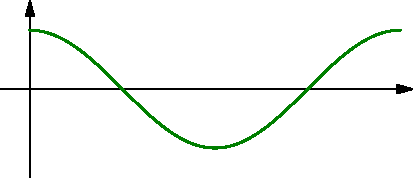
\includegraphics{./C2004_7.pdf}
 \caption{Représentation graphique de $\cos$ restreinte à $\left[0 , 2\pi \right]$.}
 \label{fig:graph1}
\end{figure}

Pour une fonction $f$ définie dans $I$ et à valeurs réelles, 
\[
 \left\lbrace (x,f(x), x\in I\right\rbrace \subset \R^2
\]
est appelé le graphe (ou la représentation graphique de $f$.\newline
En se donnant une fonction $f$ et un réel $a>0$, on définit dans le tableau suivant de nouvelles fonctions et des \emph{transformations affines} \index{transformations affines} du plan $\R^2$. \index{symétrie axiale} \index{affinité}
\begin{center}
\renewcommand{\arraystretch}{1.5}
\begin{tabular}{|c|c|c|c|c|c|} \hline
fonction (image de $x$)& $f(x) +a$ & $ f(x+a)$ & $ f(a-x)$ & $ f(ax)$ & $ af(x)$\\ \hline
transformation (image de $(x,y)$)& $(x,y+a)$ & $(x-a,y)$ & $(a-x,y) $ & $(\frac{x}{a},y)$ & $(x,ay)$\\ \hline
type transformation & translation & translation & symétrie axiale & affinité & affinité \\ \hline
\end{tabular}
\end{center}
Il faut bien noter que ces fonctions ne sont pas forcément définies dans le même ensemble de départ. Le graphe de chacune est l'image du graphe de la fonction initiale par la transformation associée. Présentons ces graphes pour le $\cos$ avec $a=1.5$.
\begin{figure}[h]
  \centering
  \subfloat[$x \mapsto f(x) + a$.]{
     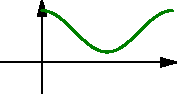
\includegraphics[width=3cm]{./C2004_8.pdf}
  }
  \subfloat[$x \mapsto f(x + a)$.]{
     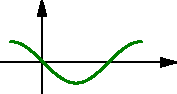
\includegraphics[width=3cm]{./C2004_9.pdf}
  }
  \subfloat[$x \mapsto f(a-x)$.]{
    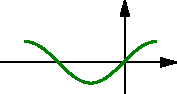
\includegraphics[width=3cm]{./C2004_10.pdf}
  }
  \subfloat[$x \mapsto f(ax)$.]{
    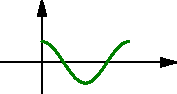
\includegraphics[width=3cm]{./C2004_11.pdf}
  }
  \subfloat[$x \mapsto af(x)$.]{
    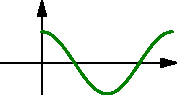
\includegraphics[width=3cm]{./C2004_12.pdf}
  }
  \caption{Graphes et transformations.}
\end{figure}


\subsubsection{Opérations}
On peut définir des opérations sur les ensembles de fonctions définies \emph{dans le même intervalle de définition}.\newline
Soit $f$ et $g$ définie dans un intervalle $I$, on définit de nouvelles fonctions somme $f+g$, produit $fg$, $\sup(f,g)$, $\inf(f,g)$, $f^{+}$, $f^{-}$, $|f|$ en présentant dans un tableau l'image d'un réel $x\in I$ quelconque
\begin{center}
\renewcommand{\arraystretch}{1.5}
\begin{tabular}{|c|c|c|c|c|c|c|} \hline
$f+g$ & $fg$ & $sup(f,g)$ & $inf(f,g)$ & $f^+$ & $f^-$ & $|f|$ \\ \hline
$f(x) + g(x)$ & $f(x)g(x)$ & $\max(f(x),g(x)$ & $\min(f(x),g(x)$ & $\max(f(x),0)$ & $\min(-f(x),0)$ & |f(x)| \\ \hline
\end{tabular}
\end{center}
Les formules suivantes sont souvent utiles.
\begin{displaymath}
 \sup(f,g) = \frac{1}{2}\left( f + g + |f-g|\right), \hspace{0.5cm}  
 \inf(f,g) = \frac{1}{2}\left( f + g - |f-g|\right).
\end{displaymath}
Attention, la composition est une opération très différente.
\subsubsection{Parité, imparité}
\index{fonction paire} \index{fonction impaire}
\begin{defi}
 Soit $f$ une fonction définie dans un intervalle $I$ symétrique par rapport à l'origine.
 \begin{itemize}
  \item La fonction $f$ est \emph{paire} si et seulement si 
  \begin{displaymath}
   \forall x\in I, \; f(-x) = f(x).
  \end{displaymath}
  \item La fonction $f$ est \emph{impaire} si et seulement si 
  \begin{displaymath}
   \forall x\in I, \; f(-x) = f(-x).
  \end{displaymath}
 \end{itemize}
\end{defi}
\begin{prop}
 Toute fonction définie dans $\R$ et à valeurs réelles se décompose de manière unique comme la somme d'une fonction paire et d'une fonction impaire.
\end{prop}
\begin{demo}
 La démonstration se fait par analyse-synthèse\index{analyse-synthèse}. Notons $f$ la fonction à décomposer.\newline
Analyse. Si $f=g+h$ avec $h$ paire et $f$ impaire alors, en écrivant cette somme pour $x$ et $-x$ et en combinant, il vient :
\begin{align*}
 g(x)=\dfrac{1}{2}(f(x)+f(-x)) &,& g(x)=\dfrac{1}{2}(f(x)-f(-x))
\end{align*}
Ceci assure l'unicité de la décomposition.\newline
Synthèse. \emph{Définissons} des fonctions $g$ et $h$ par les formules :
\begin{align*}
 g(x)=\dfrac{1}{2}(f(x)+f(-x)) &,& g(x)=\dfrac{1}{2}(f(x)-f(-x))
\end{align*}
On vérifie alors facilement que $g$ est paire, $h$ impaire et $f=g+h$. Ce qui assure l'existence d'une décomposition. 
\end{demo}
Les symétries dans le graphe d'une fonction définie dans $\R$ généralisent la parité et l'imparité.
Deux réels $x$ et $x'$ sont symétriques par rapport à un réel $a$ si et seulement si $x+x' = 2a$ (le point $a$ est le milieu des deux). De même deux points de coordonnées $(x,y)$ et $(x',y')$ sont symétriques (symétrie centrale) \index{symétrie centrale} par rapport au point de coordonnées $(a,b)$ si et seulement si 
\begin{displaymath}
 x + x' = 2a, \hspace{0.5cm} y + y' = 2b.
\end{displaymath}
On en déduit que 
\begin{itemize}
 \item le graphe de $f$ est symétrique (symétrie centrale) par rapport au point $(a,f(a))$ si et seulement si 
\begin{displaymath}
\forall x \in \R, \; f(x) + f(2a-x) = 2f(a) 
\end{displaymath}
 \item le graphe de $f$ est symétrique (symétrie axiale) par rapport à la droite d'équation $x = a$ si et seulement si 
\begin{displaymath}
\forall x \in \R, \; f(2a-x) = f(x) 
\end{displaymath}
\end{itemize}

\subsubsection{Périodicité}
\begin{defi}
Soit $f$ une fonction définie dans $\R$ et $T\in \R$. On dit que $T$ est une \emph{période} de $f$ si et seulement si 
\begin{displaymath}
 \forall x\in \R, \; f(x+T) = f(x)
\end{displaymath}
On dit que $f$ est périodique si et seulement si il existe une période \emph{non nulle} de $f$. 
\end{defi}
\begin{rem}
 Si $f$ est périodique et $\mathcal{T}$ est l'ensemble de ses périodes alors $\mathcal{T}$ est un sous-groupe additif de $\R$ c'est à dire
\begin{displaymath}
 \forall (T,T')\in \mathcal{T}^2, \; T+T' \in \mathcal{T},\; -t\in \mathcal{T}.
\end{displaymath}
\end{rem}

\subsubsection{Monotonie}
\begin{defi}
 Une fonction $f$ définie dans un intervalle $I$ est 
\begin{itemize}
 \item croissante si et seulement si $\forall (x,y)\in I^2\; x < y \Rightarrow f(x) \leq f(y)$,
 \item strictement croissante si et seulement si $\forall (x,y)\in I^2\; x < y \Rightarrow f(x) < f(y)$,
 \item décroissante si et seulement si $\forall (x,y)\in I^2\; x < y \Rightarrow f(y) \leq f(x)$,
 \item strictement décroissante si et seulement si $\forall (x,y)\in I^2\; x < y \Rightarrow f(y) < f(x)$,
 \item monotone si et seulement si elle est croissante ou décroissante,
 \item strictement monotone si et seulement si elle est strictement croissante ou strictement décroissante.
\end{itemize}
\end{defi}
\begin{rem}
 Une fonction strictement monotone est injective. La réciproque n'est pas vraie sans hypothèse supplémentaire (continuité) comme le montre (figure \ref{fig:C2004_6}) l'exemple de la fonction
\begin{displaymath}
 \left\lbrace 
 \begin{aligned}
  \left[ 0 , 1\right] &\rightarrow \left[ 0 , 1\right]\\
  x &\mapsto
      \left\lbrace 
          \begin{aligned}
          x                &\text{ si } 0 \leq x \leq \frac{1}{2} \\
          \frac{3}{2} - x  &\text{ si } \frac{1}{2} < x < 1 \\
          1               &\text{ si } x = 1
          \end{aligned}    
      \right. 
  \end{aligned}
  \right. 
\end{displaymath}
\end{rem}
\begin{figure}[h]
 \centering
 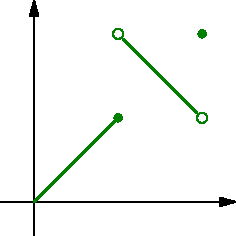
\includegraphics{./C2004_6.pdf}
 % C2004_6.pdf: 0x0 pixel, 0dpi, 0.00x0.00 cm, bb=
 \caption{Fonction injective non monotone}
 \label{fig:C2004_6}
\end{figure}

\begin{prop}
 Soit $f$ définie dans un intervalle $I$ et $g$ définie dans un intervalle $J$ tel que $f(I)\subset J$. Si $f$ et $g$ sont monotones (resp strictement) alors $g\circ f$ est monotone (resp strictement). Le sens de monotonie est donné par le tableau suivant
\begin{center}
\renewcommand{\arraystretch}{1.3}
\begin{tabular}{|c|c|c|}  \hline
$f$          & $g$          & $g\circ f$\\ \hline
croissante   & croissante   & croissante\\ \hline
croissante   & décroissante & décroissante\\ \hline
décroissante & croissante   & décroissante\\ \hline
décroissante & décroissante & croissante\\ \hline
\end{tabular}
\end{center}
\end{prop}

\subsubsection{Fonctions majorées, minorées, bornées}
\begin{defi}
 Une fonction $f$ définie dans un intervalle $I$ est \emph{majorée}(resp \emph{minorée}, \emph{bornée}) si et seulement si $f(I)$ est majoré(resp minoré, borné). 
\end{defi}
\begin{rems}
\begin{itemize}
 \item $f(I)$ désigne l'ensemble des images par $f$ au sens de l'image directe d'une partie par une fonction.
 \item Une fonction à valeurs réelles $f$ est bornée si et seulement si $|f|$ est majorée.
\end{itemize}
\end{rems}
Opérations sur les fonctions bornées : à compléter.


 \index{théorème des valeurs intermédiaires}
\subsection{Théorème de la valeur intermédiaire}
\begin{thm}[Théorème de la valeur intermédiaire]
 \begin{description}
  \item[formulation 1]Soit $I$ un intervalle et $a, b$ dans $I$ tels que $a<b$. Soit $f$ une fonction continue sur $I$ telle que $f(a)f(c)<0$. Il existe alors $c$ tel que $f(c)=0$.
  \item[formulation 2]Soit $I$ un intervalle, $a\in I$, $b\in I$, $f$ continue sur $I$ et $\lambda \in ]\min(f(a),f(b)),\max(f(a),f(b))[$. Il existe alors $c\in[\min(a,b),\max(a,b)]$ tel que $f(c)=\lambda$.
  \item[formulation 3]Soit $I$ un intervalle et $f$ une fonction continue sur $I$. Alors $f(I)$ est un intervalle.
 \end{description}
\end{thm}
voir \href{\baseurl C2072.pdf}{Propriétés globales des fonctions continues.}
\begin{rem}
Le théorème des valeurs intermédiaires est liée à la surjectivité. Il montre par exemple que si $f$ est continue dans $I$ et à valeurs dans $[m,M]$, et s'il existe $u$, $v$ dans $I$ tels que $f(u)=m$, $f(v) = M$, alors la fonction est surjective. 
\end{rem}

\section{Dérivation}
Les résultats seront démontrés dans la section \href{\baseurl C2070.pdf}{Propriétés globales des fonctions dérivables}
\begin{figure}[h]
 \centering
 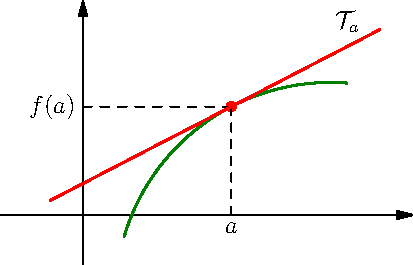
\includegraphics{./C2004_13.pdf}
 % C2004_tan.pdf: 0x0 pixel, 0dpi, 0.00x0.00 cm, bb=
 \caption{Tangente au graphe}
 \label{fig:tan}
\end{figure}

\subsection{Tangente}
Tangente au graphe, équation de la tangente.\index{équation de la tangente}
\begin{prop}
 Soit $f$ une fonction dérivable dans un intervalle $I$ et $a\in I$. L'équation de la tangente au point $(a,f(a))$ au graphe de $f$ est
\begin{displaymath}
 y - f(a) = f'(a)(x-a)
\end{displaymath}
\end{prop}
Si on note $\mathcal{T}_a$ cette tangente (figure \ref{fig:tan}), cela signifie qu'un point $M$ de coordonnées $(x,y)$ appartient à $\mathcal{T}_a$ si et seulement si $y-f(a) = f'(a)(x-a)$.

\subsection{Opérations}
\begin{prop}[somme et produit]
Soit $f$ et $g$ des fonctions dérivables sur un intervalle $I$ et $\lambda\in \R$. Les fonctions $f+g$, $\lambda f$, $fg$ sont dérivables avec
\begin{displaymath}
 (f+g)' = f' + g',\hspace{0.5cm} (\lambda f)' = \lambda f',\hspace{0.5cm} (fg)' = f'g + f g'
\end{displaymath}
\end{prop}

\begin{prop}[composée]
 Soit $f$ dérivable dans un intervalle $I$ et $g$ dérivable dans un intervalle $J$ tel que $f(I)\subset J$. La fonction $g \circ f$ est dérivable dans $I$ et vérifie
\begin{displaymath}
 (g \circ f)' = f'\, g'\circ f.
\end{displaymath}
\end{prop}

\begin{prop}[puissance]
 Pour les hypothèses présentées dans le tableau suivant
\begin{center}
\renewcommand{\arraystretch}{1.5}
\begin{tabular}{|c|c|c|c|} \hline
$\alpha$       & $\N$ & $-\N$  & $\C$ \\ \hline
valeurs de $f$ & $\R$ & $\R^*$ & $\left] 0, +\infty\right[$ \\ \hline
\end{tabular}
\end{center}
 
 la fonction $f^{\alpha}$ est dérivable et vérifie
\begin{displaymath}
 (f^{\alpha})' = \alpha f' f^{\alpha -1}
\end{displaymath}
\end{prop}

\begin{rems}
 \begin{itemize}
  \item La dérivation des fonctions à valeurs complexes est présentée à la fin de ce chapitre.
  \item Volontairement, je ne présente pas de formule pour le quotient de deux fonctions. Je n'aime pas cette formule car elle donne à penser que l'exposant du dénominateur est doublé alors qu'il augmente seulement de $1$. Dériver comme un produit de puissances est une meilleure pratique.
  \begin{displaymath}
   (\frac{f}{g^m})' = \frac{f'}{g^m} - m \, \frac{fg'}{g^{m+1}}
  \end{displaymath}
 \end{itemize}
\end{rems}

\subsection{Tableau de variations}
\index{théorème du tableau de variations}
\begin{thm}[théorème du tableau de variations]
 Soit $f$ une fonction continue dans $[a,b]$, dérivable dans $]a,b[$ telle que $f'(x)>0$ pour tout $x\in]a,b[$. Alors $f$ est strictement croissante dans $[a,b]$.
\end{thm}
voir \href{\baseurl C2070.pdf}{Propriétés des fonctions dérivables.} En considérant $-f$, on montre que si $f'<0$ la fonction est strictement décroissante..
On peut combiner avec le théorème des valeurs intermédiaires pour obtenir une condition suffisante de bijectivité. Il vaut mieux les appliquer séparément et comprendre que le théorème du tableau des variations est lié à l'\emph{injectivité} alors que le théorème des valeurs intermédiaires est lié à la \emph{surjectivité}. 
\begin{prop}[caractérisation des fonctions dérivables constantes]
 Une fonction dérivable dans un intervalle est constante si et seulement si sa dérivée est nulle.
\end{prop}


\subsection{Dérivabilité d'une bijection réciproque}
 \index{dérivabilité d'une bijection réciproque}
\begin{thm}[dérivabilité d'une bijection réciproque]
 Soit $f$ une fonction continue dans $[a,b]$, dérivable dans $]a,b[$ telle que $f'(x)>0$ pour tout $x\in]a,b[$, alors $f$ est bijective de $[a,b]$ dans $[f(a),f(b)]$, sa bijection réciproque est continue dans $[f(a),f(b)]$, dérivable dans $]f(a),f(b)[$ avec :
\begin{displaymath}
 \forall y \in \left]f(a),f(b)\right[ : {f^{-1}}^\prime(y) = \dfrac{1}{f'(g(y))}
\end{displaymath}
\end{thm}
voir \href{\baseurl C2070.pdf}{Propriétés des fonctions dérivables.}
\begin{rem}
 Le graphe de la fonction réciproque de $f$ est obtenu par symétrie par rapport à la première bissectrice. En effet, si $(x,y)$ est un point du graphe de $f$, alors le symétrique de ce point par rapport à la première bissectrice est $(y,x)$. Or, comme $f$ est bijective,
 \begin{displaymath}
  (x,y)\in\text{ graphe de $f$} \Leftrightarrow y = f(x)
  \Leftrightarrow x = f^{-1}(y) \Leftrightarrow (y,x) \in \text{ graphe de $f^{-1}$}
 \end{displaymath}
\end{rem}
On peut supposer $f'<0$ dans ce cas, l'intervalle de définition de la bijection réciproque est $\left]f(b),f(a)\right[$.

\subsection{Dérivées successives}
Lorsqu'une fonction est dérivable, sa dérivée peut être elle même dérivable. On dit alors que la fonction est deux fois dérivable.\newline
On utilise des puissances symboliques pour désigner les dérivées successives. Par exemple pour la dérivée seconde $f^{(2)} = f''$.\newline
Pour tout entier naturel $n$, on dit qu'une fonction est $n+1$ fois dérivable si et seulement si elle $n$ fois dérivable et que sa dérivée d'ordre $n$ est dérivable. On note
\[
 \left( f^{(n)}\right)' = f^{(n+1)}. 
\]
On note $\mathcal{D}^{k}(I,\R)$ l'ensemble des fonctions $k$ fois dérivables dans $I$ et $\mathcal{C}^{k}(I,\R)$ celles qui sont $k$ fois dérivables et dont la dérivée d'ordre $k$ est continue. On a alors une succession d'inclusions(pour des fonctions définies dans un même intervalle $I$)
\[
\mathcal{C}^{+\infty} \subset \cdots \subset \mathcal{C}^{k} \subset \mathcal{D}^{k} \subset \mathcal{C}^{k-1} \subset \mathcal{D}^{k-1} \subset \cdots \subset \mathcal{C}^{1} \subset \mathcal{D}^{1}\subset \mathcal{C}^{0}.
\]
où $\mathcal{C}^{+\infty}$ désigne l'ensemble des fonctions infiniment (ou indéfiniment) dérivables. Toutes les dérivées successives sont alors continues.

\section{Fonctions usuelles}
\subsection{Autour de la fonction exponentielle réelle}
\subsubsection{Fonction logarithme}
\begin{prop}
 La fonction  \hyperdef{prop}{expreelle}{exponentielle réelle} est une bijection strictement croissante de $\R$ dans $\R_+^*$.
\end{prop}
\begin{demo}
Par définition, le fonction exponentielle ne prend pas la valeur nulle. Deplus, pour tout $t$ réel :
\begin{displaymath}
 \exp(t)=(\exp(\dfrac{t}{2}))^2>0
\end{displaymath}
car c'est le carré d'un nombre réel. De plus d'après la propriété P4, la fonction exponentielle réelle est dérivable et elle est égale à sa dérivée donc strictement positive. On en déduit que la fonction est strictement croisante dans $\R$. Montrons que sa limite en $+\infty$ est $+\infty$. Notons $e=\exp(1)$. \`A cause de la stricte croissance, $e>1$ donc $\left(e^n \right)_{n\in\N}$ est une suite géométrique de raison $>1$ donc divergente vers $+\infty$. On en déduit que 
$\left(e^n \right)_{n\in\N}$ puis la fonction (car elle est croissante) diverge vers $+\infty$.
\end{demo}

\index{définition du logarithme}
\begin{defi}[Définition du logarithme]
La fonction logarithme notée $\ln$ est la bijection réciproque de la fonction exponentielle réelle.
\end{defi}
Les résultats cités dans le glossaire relatifs à la dérivabilté d'un bijection réciproque prouve la proposition suivante.
\begin{prop}
 La fonction $\ln$ est dérivable dans $]0,+\infty[$ avec $\ln'(x)=\frac{1}{x}$ pour tout $x>0$.
\end{prop}

limites usuelles \index{limites usuelles}
En particulier $\frac{\ln x}{x}\rightarrow 0$ en $+\infty$ en $+\infty$. On en déduit $\frac{1}{x}e^x\rightarrow +\infty$.
\begin{demo} à compléter
  La démonstration des valeurs de ces limites est un exemple d'utilisation d'une étude de fonction. La fonction que l'on étudie est 
  \begin{displaymath}
    x \mapsto \ln x - 2\sqrt{x}
  \end{displaymath}
\end{demo}

\subsubsection{Trigonométrie hyperbolique}
\index{définition du cosinus hyperbolique}\index{définition du sinus hyperbolique}
\begin{defi}
 La fonction sinus hyperbolique (notée $\sh$) est la partie impaire de la fonction exponentielle réelle.\\
La fonction cosinus hyperbolique (notée $\ch$) est la partie paire de la fonction exponentielle réelle.
\begin{displaymath}
  \ch x = \frac{1}{2}(e^{x} + e^{-x}),\hspace{1cm} \sh x = \frac{1}{2}(e^{x} - e^{-x})
\end{displaymath}
\end{defi}
Propriétés : $e^{x} =  \ch x + \sh x$, $e^{-x} = \ch x - \sh x$, $\ch^2x - \sh^2 x = 1$. 
Justification du terme par paramétrisation d'une branche d'hyperbole.\index{hyperbole}
\begin{figure}[h]
  \centering
  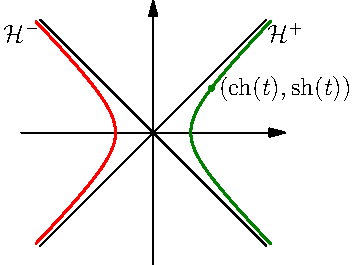
\includegraphics{./C2004_4.pdf}
  \caption{Paramétrisation d'une hyperbole}
  \label{fig:C2004_4}
\end{figure}
\begin{figure}[h]
  \centering
  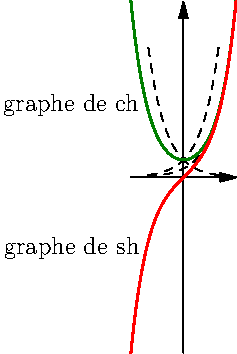
\includegraphics{./C2004_5.pdf}
  \caption{Graphes de $\ch$ et $\sh$.}
  \label{fig:C2004_5}
\end{figure}

\subsection{Trigonométrie circulaire}

\subsubsection{Conséquences de la présentation axiomatique de l'exponentielle}
\begin{prop}
 La restriction de la fonction $\cos$ à l'intervalle $[0,\pi]$ est strictement décroissante, la fonction $\sin$ est strictement positive dans $]0,\pi[$.
\end{prop}
\begin{demo}
 On a vu dans le cours sur les complexes que 
\begin{displaymath}
 \sin x= 0 \Leftrightarrow x\in \pi \Z
\end{displaymath}
On en déduit que $\sin$ ne s'annule pas dans $]0,\pi[$. Or d'après P4, la dérivée de $\cos$ est $-\sin$. On en déduit que $\cos$ est strictement monotone dans $[0,\pi]$. Or on sait que $\cos 0=0$ et $\cos \pi =-1$. On en déduit que $\cos$ est strictement décroissant dans $[0,\pi]$ et que $\sin$ est strictement positif dans $]0,\pi[$.
\end{demo}

\begin{prop}[\hyperdef{prop}{surjexp}{Surjectivité de la fonction exponentielle}]
Pour tout nombre complexe non nul $z$, il existe des nombres complexes $u$ tels que $\exp(u)=z$.\newline
Pour tout nombre complexe de module $1$, il existe des nombres réels $y$ tels que $\exp(iy)=u$.
\end{prop}
\begin{demo}
On commence par montrer que pour tout nombre complexe $u$ de module $1$, il existe un réel $y$ tel que $u=\exp(y)$.\newline
Comme $|u|^2=(\Re u)^2+(\Im u)^2=1$, on a $\Re u\in [-1,+1]$. D'après le tableau de variation de la restriction de $\cos$ à $[0,\pi]$, il existe $t\in[0,\pi]$ tel que $\cos t = \Re u$. Les sommes de carrés sont égales à 1 donc
$\Im u \in \{\sin t , -\sin t\}$. Or $\cos(-t)=\cos t$ et $\sin (-t)=-\sin t$. Il existe donc $y\in\{t, -t\}$ tel que
\begin{displaymath}
 u=\exp(y)
\end{displaymath}
Passons au cas général où $z$ est un complexe non nul. D'après les propriétés de l'exponentielle réelle, il existe un réel $x$ tel que $\exp(x)=|z|$. D'après ce que l'on vient de montrer, il existe un réel $y$ tel que
\begin{displaymath}
 \dfrac{z}{|z|}=\exp(iy)
\end{displaymath}
On en déduit
\begin{displaymath}
 \exp(x+iy)=|z|\dfrac{z}{|z|}=z
\end{displaymath}
\end{demo}

Caractérisation des nombres complexes de module 1. Pour tout nombre complexe non nul, il existe un complexe $u$ tel que $e^u$.
\begin{prop}
 Soit $a$ et $b$ deux réels tels que $(a,b)\neq(0,0)$. Il existe $\varphi\in\R$ tel que, 
\begin{displaymath}
 \forall x\in \R: \hspace{0.5cm} a\cos x + b\sin x = \sqrt{a^2+b^2}\cos(x+\varphi) 
\end{displaymath}
\end{prop}

\subsubsection{Formulaire}
\index{formulaire de trigonométrie circulaire}\index{formulaire de trigonométrie hyperbolique}
Dans ce formulaire, $a, b, x$ sont réels et $n$ entier relatif.
\twocolumn
\begin{center}
 Trigonométrie circulaire
\end{center}
Définitions
\begin{displaymath}
  \cos a  = \frac{1}{2}(e^{ia}+e^{-ia}) \hspace{0.5cm} \sin a  = \frac{1}{2i}(e^{ia}-e^{-ia})
\end{displaymath}
\begin{align*}
  \cos a + i \sin a  &= e^{ia}& &\text{(Euler)}\\
  (\cos a + i \sin a)^n &= \cos(na) + i \sin(na)& &\text{(Moivre)}
\end{align*}
Module
\begin{displaymath}
 (\cos a)^2 + (\sin a)^2 = 1 \hspace{0.5cm} 1+\tan^2a = \frac{1}{\cos^2 a}
\end{displaymath}
Autour de $e^{z+z'}=e^{e}e^{^{z'}}$
\begin{align*}
 &\cos(a+b) = \cos a \cos b  - \sin a \sin b\\
 &\sin(a+b) = \sin a \cos b + \cos a \sin b \\
 &\tan(a+b) = \frac{\tan a + \tan b}{1-\tan a \tan b}\\
 &\cos(2a) = \cos^2 a -\sin^2 a \\
 &         =2\cos^2 a -1 = 1-2\sin^2a\\
 &\sin(2a) = 2\sin a \cos a \\
 &\tan(2a) = \frac{2\tan a }{1-\tan^2 a}
\end{align*}
Symétries

$\sin$ et $\cos$ sont $2\pi$ périodiques.

$\sin$ impaire, $\cos$ paire.
\begin{align*}
  &\cos(a+\pi) = -\cos a & & \cos (\pi-a) = -\cos a \\
  &\sin(a+\pi) = -\sin a & & \sin (\pi-a) = \sin a \\
  &\tan(a+\pi) = \tan a & & \tan (\pi-a) = -\tan a \\
  &\cos(\frac{\pi}{2}-a) = \sin a & & \cos(\frac{\pi}{2}+a) = -\sin a\\ 
  &\sin(\frac{\pi}{2}-a) = \cos a & & \sin(\frac{\pi}{2}+a) = \cos a\\ 
  &\tan(\frac{\pi}{2}-a) = \frac{1}{\tan a } & & \tan(\frac{\pi}{2}+a) = -\frac{1}{\tan a}\\ 
\end{align*}
Expression avec la tangente de l'arc moitié.\newline
Pour $a\not \equiv \pi \mod (2\pi)$ et $t = \tan \frac{a}{2}$
\begin{align*}
 \cos a  = \frac{1-t^2}{1+t^2} & &
  \sin a = \frac{2t}{1+t^2} & &
  \tan a = \frac{2t}{1-t^2} 
\end{align*}
Produit $\rightarrow$ Somme (linéarisation)
\begin{align*}
 &\cos a \cos b = \frac{1}{2}\left(\cos(a-b) +\cos(a+b)\right)\\
 &\sin a \sin b = \frac{1}{2}\left(\cos(a-b)-\cos(a+b) \right)\\
 &\sin a \cos b = \frac{1}{2}\left(\sin(a-b)+\sin(a+b) \right) \\
 &\cos^2 a = \frac{1}{2}+\frac{1}{2}\cos(2a)\\
 &\sin^2 a = \frac{1}{2}-\frac{1}{2}\cos(2a)
\end{align*}
Somme $\rightarrow$ Produit (factorisation)
\begin{align*}
 &\cos a + \cos b = 2\cos \frac{a+b}{2} \cos \frac{a-b}{2} \\  
 &\cos a - \cos b = -2\sin \frac{a+b}{2} \sin \frac{a-b}{2} \\
 &\sin a + \sin b = 2\sin \frac{a+b}{2} \cos \frac{a-b}{2}
\end{align*}
\'Equations
\begin{align*}
 &\sin x = 0 &\Leftrightarrow x \equiv 0 \mod(\pi) \\
 &\cos x = 0 &\Leftrightarrow x \equiv \frac{\pi}{2} \mod(\pi) \\
 &\sin x = \sin a &\Leftrightarrow
\left\lbrace 
\begin{aligned}
 &x \equiv a \mod(2\pi)\\
&\text{ ou }\\
 &x \equiv \pi - a \mod(2\pi)
\end{aligned}
\right. \\
 &\cos x = \cos a &\Leftrightarrow
\left\lbrace 
\begin{aligned}
 &x \equiv a \mod(2\pi)\\
&\text{ ou }\\
 &x \equiv  - a \mod(2\pi)
\end{aligned}
\right. 
\end{align*}

\begin{center}
\hrulefill \\ 
 Trigonométrie hyperbolique
\end{center}

$\ch$ est la partie \emph{paire} de l'exponentielle réelle.

$\sh$ est la partie \emph{impaire} de l'exponentielle réelle.

\begin{align*}
 &e^{a} = \ch a + \sh a &  &e^{-a} = \ch a - \sh a \\
 &\ch a = \frac{1}{2}\left( e^a + a^{-a}\right)  & & \sh a = \frac{1}{2}\left( e^a - a^{-a}\right)
\end{align*}

\begin{displaymath}
 (\ch a)^2 - (\sh a)^2 = 1
\end{displaymath}

\begin{align*}
 &\ch(a+b) = \ch a \ch b  + \sh a \sh b\\
 &\sh(a+b) = \sh a \ch b + \ch a \sh b \\
 &\th(a+b) = \frac{\th a + \th b}{1+\th a \th b}\\
 &\ch(2a) = (\ch a)^2 + (\sh a)^2 \\
 &\sh(2a) = 2\sh a \ch a \\
 &\th(2a) = \frac{2\th a }{1+\th^2 a}
\end{align*}

\onecolumn
\clearpage
\subsubsection{Calculs trigonométriques}
Exemples de linéarisation $\sin^2x\cos^3 x$, $ \cos x \cos2x \cos 3x$. Utilisation de le formule du binôme pour linéariser $\sin^5x$ ou $\cos^6 x$.
\index{linéarisation}
\begin{figure}[h!t]
 \centering
 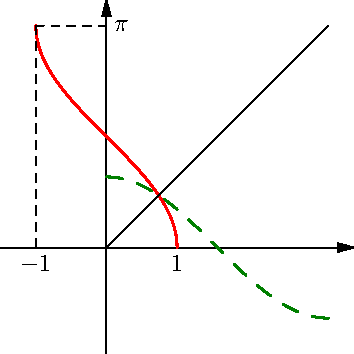
\includegraphics{./C2004_1.pdf}
 % C2004_1.pdf: 0x0 pixel, 0dpi, 0.00x0.00 cm, bb=
 \caption{Graphe de $\arccos$}
 \label{fig:C2004_1}
\end{figure}
\begin{figure}[h!t]
 \centering
 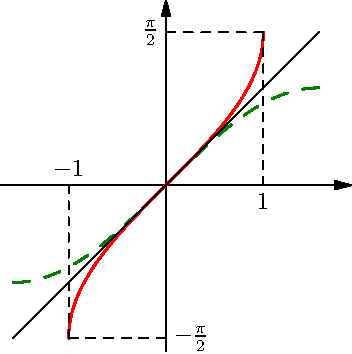
\includegraphics{./C2004_2.pdf}
 % C2004_1.pdf: 0x0 pixel, 0dpi, 0.00x0.00 cm, bb=
 \caption{Graphe de $\arcsin$}
 \label{fig:C2004_2}
\end{figure}
\begin{figure}[h!t]
 \centering
 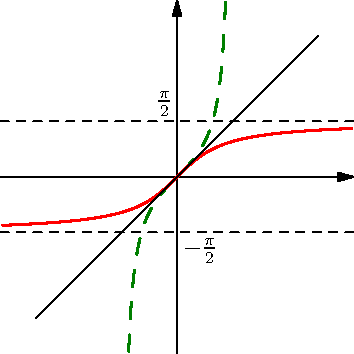
\includegraphics{./C2004_3.pdf}
 % C2004_1.pdf: 0x0 pixel, 0dpi, 0.00x0.00 cm, bb=
 \caption{Graphe de $\arctan$}
 \label{fig:C2004_3}
\end{figure}

\subsubsection{Fonctions réciproques}
\index{définition de $\arccos$}
\begin{defi}[fonction $\arccos$]
 La fonction
\begin{displaymath}
 \left(
\begin{aligned}
 \left[ 0,\pi\right]   &\rightarrow [-1,1]\\x &\mapsto \cos x
\end{aligned}
\right. 
\end{displaymath}
est bijective. Sa bijection réciproque est la fonction $\arccos$.
\end{defi}

\index{définition de $\arcsin$}
\begin{defi}[fonction $\arcsin$]
 La fonction
\begin{displaymath}
 \left(
\begin{aligned}
 \left[ -\frac{\pi}{2},\frac{\pi}{2}\right]   &\rightarrow [-1,1]\\x &\mapsto \sin x
\end{aligned}
\right. 
\end{displaymath}
est bijective. Sa bijection réciproque est la fonction $\arcsin$.
\end{defi}

\index{définition de $\arctan$}
\begin{defi}[fonction $\arctan$]
 La fonction
\begin{displaymath}
 \left(
\begin{aligned}
 \left] -\frac{\pi}{2},\frac{\pi}{2}\right[   &\rightarrow \R \\x &\mapsto \tan x
\end{aligned}
\right. 
\end{displaymath}
est bijective. Sa bijection réciproque est la fonction $\arctan$.
\end{defi}

Caractérisation. Il faut retenir qu'une égalité $\theta$ = arcquelque chose se traduit par DEUX relations.
\begin{displaymath}
 \theta = \arccos(x)\Leftrightarrow
\left\lbrace 
\begin{aligned}
 &\theta \text{ a le bon } \cos \\ &\theta \text{ est dans le bon intervalle}
\end{aligned}
\right. 
\Leftrightarrow
\left\lbrace 
\begin{aligned}
 &\cos \theta = x \\ &\theta \in [0,\pi]
\end{aligned}
\right. 
\end{displaymath}

\begin{displaymath}
 \theta = \arcsin(x)\Leftrightarrow
\left\lbrace 
\begin{aligned}
 &\theta \text{ a le bon } \sin \\ &\theta \text{ est dans le bon intervalle}
\end{aligned}
\right. 
\Leftrightarrow
\left\lbrace 
\begin{aligned}
 &\sin \theta = x \\ &\theta \in \left[ -\frac{\pi}{2},\frac{\pi}{2}\right] 
\end{aligned}
\right. 
\end{displaymath}

\begin{displaymath}
 \theta = \arctan(x)\Leftrightarrow
\left\lbrace 
\begin{aligned}
 &\theta \text{ a la bonnne } \tan \\ &\theta \text{ est dans le bon intervalle}
\end{aligned}
\right. 
\Leftrightarrow
\left\lbrace 
\begin{aligned}
 &\tan \theta = x \\ &\theta \in \left] -\frac{\pi}{2},\frac{\pi}{2}\right[ 
\end{aligned}
\right. 
\end{displaymath}
\begin{rem}
  On peut utiliser la fonction $\arctan$ pour exprimer un argument d'un nombre complexe $z$ qui n'est pas imaginaire pur:
\begin{align*}
  &\text{si } \Re(z)>0 \text{ un argument de $z$ est } &\arctan\frac{\Im(z)}{\Re(z)} \\
  &\text{si } \Re(z)<0 \text{ un argument de $z$ est } &\pi + \arctan\frac{\Im(z)}{\Re(z)} 
\end{align*}
\end{rem}


Les résultats présentés dans la section sur les fonctions dérivables et relatifs à la dérivabilité des bijections réciproques montrent les résultats suivants.
\begin{prop}
 La fonction $\arccos$ est dérivable dans $]0,\pi[$ avec
\begin{displaymath}
 \forall x \in ]0,\pi[,\hspace{0.5cm}
\arccos'(x) = -\frac{1}{\sqrt{1-x^2}}
\end{displaymath}
La fonction $\arcsin$ est dérivable dans $\left] -\frac{\pi}{2}, \frac{\pi}{2}\right[$ avec
\begin{displaymath}
 \forall x \in \left] -\frac{\pi}{2}, \frac{\pi}{2}\right[,\hspace{0.5cm}
\arcsin'(x) = \frac{1}{\sqrt{1-x^2}}
\end{displaymath}
La fonction $\arctan$ est dérivable dans $\R$ avec
\begin{displaymath}
 \forall x \in \R,\hspace{0.5cm}
\arctan'(x) = \frac{1}{1+x^2}
\end{displaymath}
\end{prop}

\begin{rems}
 \begin{enumerate}
\item Deux démonstrations de la formule
\begin{displaymath}
 \forall x \in [-1,1],\hspace{0.5cm}\arccos x + \arcsin x = \frac{\pi}{2}
\end{displaymath}
en utilisant $\frac{\pi}{2}-a$, en dérivant. à compléter
 \item graphe de $\arcsin \circ \sin$.\index{question de cours!graphe de $\arcsin \circ \sin$} à compléter, faire un dessin 
  \item Si $z$ est un nombre complexe de partie réelle strictement positive, $\arctan \frac{\Im(z)}{\Re(z)}$ est un argument de $z$. On peut remarquer que dans ce cas $w= \ln |z|+i\arctan \frac{\Im(z)}{\Re(z)}$ est un antécédent de $z$ pour la fonction exponentielle complexe. Si la partie réelle de $z$ est strictement négative, $\pi +\arctan \frac{\Im(z)}{\Re(z)}$ est un argument de $z$.
 \end{enumerate}
\end{rems}

\section{Dérivation d'une fonction d'une variable réelle à valeurs complexes}
\begin{defi}
Soit $f$ une fonction définie dans un intervalle $I$ de $\R$ dont les fonctions $\Re(f)$ et $\Im(f)$ sont dérivables, alors $f$ est dérivable avec
\begin{displaymath}
  f' = \left( \Re(f)\right)' + i\left( \Im(f)\right)'  
\end{displaymath}
\end{defi}
Les formules usuelles sont valables pour des fonctions à valeurs complexes et dérivables
\begin{displaymath}
  (\overline{f\strut})' = \overline{f'\strut}, \hspace{0.5cm} (f+g)' = f' +g', \hspace{0.5cm} (fg)' = f'g + fg', \hspace{0.5cm} n\in \N, (f^n)' = nf'f^{n-1}
\end{displaymath}
Lorsque $f$ ne s'annule pas, cela se généralise à $n\in \Z$. Attention, on ne peut étendre à des exposants complexes que lorsque $f$ est à valeurs strictement positives. Les fonctions d'une variable réelle $t$ qui s'expriment à l'aide de fractions formées avce des polynômes à coefficients complexes se dérivent donc selon les formules usuelles.\newline
On peut déduire la proposition suivante de la définition axiomatique de la fonction exponentielle complexe
\begin{prop}
  Soit $\varphi$ dérivable de $I$ dans $\C$, alors la fonction $\exp \circ \varphi$ est dérivable  de dérivée
  \begin{displaymath}
    t \mapsto \varphi'(t)e^{\varphi(t)}
  \end{displaymath}
\end{prop}
En particulier, pour $\lambda\in C$ fixé, la fonction de $\R$ dans $\C$ définie par $t\mapsto e^{\lambda t}$ est dérivable de dérivée $t\mapsto \lambda e^{\lambda t}$. Attention, on ne dispose d'aucun résultat si on veut remplacer la fonction $\exp$ complexe par une autre fonction de $\C$ dans $\C$. On ne connait même pas de définition d'une \og dérivabilité\fgé d'une telle fonction.\newline
Attention aussi à la composition:
\begin{prop}
  Soit $\varphi$ dérivable de $I$ dans $J$ (intervalles de $\R$), soit $f$ dérivable de $J$ dans $\C$, alors $f\circ \varphi$ est dérivable dans $I$ avec
  \begin{displaymath}
    (f\circ \varphi)' = \varphi' f'\circ \varphi
  \end{displaymath}
\end{prop}
On en déduit que si $f$ est une fonction à valeurs strictement positives et $z\in \C$, alors $t\mapsto f(t)^z$ est dérivable de dérivée
\begin{displaymath}
  t\mapsto z f'(t)f(t)^{z-1} 
\end{displaymath}
On en déduit en particulier que 
La proposition suivante est utile pour les calculs de primitives:
\begin{prop}
Soit $z$ un complexe non réel fixé. La fonction définie dans $\R$ et à valeurs complexes
\begin{displaymath}
 t\mapsto \ln|t+z|-i\arctan\frac{t+\Re(z)}{\Im(z)}
\end{displaymath}
est dérivable et sa fonction dérivée est
\begin{displaymath}
 t\mapsto \frac{1}{t+z}
\end{displaymath}
\end{prop}
\begin{demo}
  On note $a=\Re(z)$ et $b=\Im(z)$. Alors
\begin{displaymath}
\ln|t+z|-i\arctan\frac{t+\Re(z)}{\Im(z)}
= \frac{1}{2}\ln\left( (t+a)^2+b^2\right) - i \arctan\frac{t+a}{b}
\end{displaymath}
sa dérivée est
\begin{displaymath}
  \frac{t+a}{(t+a)^2+b^2} - \frac{i}{b}\,\frac{1}{1+(\frac{t+a}{b})^2}
  = \frac{t+a-ib}{|t+z|^2}
  = \frac{t + \overline{t}}{|t+z|^2} = \frac{1}{t+z}
\end{displaymath}
\end{demo}

Dérivée de $\exp \circ \varphi$ où $\varphi$ est une fonction d'une variable réelle et à valeurs complexes. à compléter


\section{Bonnes et mauvaises pratiques}
Pour des fonctions $f$ et $g$ définies respectivement dans des intervalles $J$ et $I$ avec $g(I)\subset J$ et dérivables dans ces intervalles.
\begin{center}
\renewcommand{\arraystretch}{2}
\begin{tabular}{|c|c|c|c|}
\hline
  Mauvaise pratique & argument & Bonne pratique & argument\\ \hline
  $f(g)$ & $g$ n'est pas un élement de $J$ &
  $f(g(x))$ désigne un réel de $f(J)$& $g(x) \in g(I) \subset J$ \\ \hline
  $f(g)$ & $g$ n'est pas un élement de $J$ &
  $f\circ g$ désigne une fonction & $g(I) \subset J$ \\ \hline 
  $(f(g))'$ & $f(g)$ ne désigne rien  &
  $(f\circ g)'$ fonction & comp. fnct. dérivables \\ \hline  
  $(f(g(x)))'$ & $f(g(x)) \in \R$ pas fonct.  &
  $(f\circ g)'(x)$ réel& valeur en $x$ \\ \hline  
\end{tabular}  
\end{center}
Le théorème de composition des fonctions dérivables s'écrit alors
\begin{align*}
  (f\circ g)' = g'\,f'\circ g &      & \text{ égalité entre des fonctions} \\
  (f\circ g)'(x) = g'(x)\,f'(g(x)) & & \text{ égalité entre des réels} \\
\end{align*}
L'opération entre $g'$ et $f'\circ g$ est une multiplication entre fonctions. Elle n'est pas marquée conformément aux conventions usuelles dans les écritures formelles.



\end{document}
